% Options for packages loaded elsewhere
\PassOptionsToPackage{unicode}{hyperref}
\PassOptionsToPackage{hyphens}{url}
%
\documentclass[
]{article}
\usepackage{amsmath,amssymb}
\usepackage{iftex}
\ifPDFTeX
  \usepackage[T1]{fontenc}
  \usepackage[utf8]{inputenc}
  \usepackage{textcomp} % provide euro and other symbols
\else % if luatex or xetex
  \usepackage{unicode-math} % this also loads fontspec
  \defaultfontfeatures{Scale=MatchLowercase}
  \defaultfontfeatures[\rmfamily]{Ligatures=TeX,Scale=1}
\fi
\usepackage{lmodern}
\ifPDFTeX\else
  % xetex/luatex font selection
\fi
% Use upquote if available, for straight quotes in verbatim environments
\IfFileExists{upquote.sty}{\usepackage{upquote}}{}
\IfFileExists{microtype.sty}{% use microtype if available
  \usepackage[]{microtype}
  \UseMicrotypeSet[protrusion]{basicmath} % disable protrusion for tt fonts
}{}
\makeatletter
\@ifundefined{KOMAClassName}{% if non-KOMA class
  \IfFileExists{parskip.sty}{%
    \usepackage{parskip}
  }{% else
    \setlength{\parindent}{0pt}
    \setlength{\parskip}{6pt plus 2pt minus 1pt}}
}{% if KOMA class
  \KOMAoptions{parskip=half}}
\makeatother
\usepackage{xcolor}
\usepackage[margin=1in]{geometry}
\usepackage{graphicx}
\makeatletter
\def\maxwidth{\ifdim\Gin@nat@width>\linewidth\linewidth\else\Gin@nat@width\fi}
\def\maxheight{\ifdim\Gin@nat@height>\textheight\textheight\else\Gin@nat@height\fi}
\makeatother
% Scale images if necessary, so that they will not overflow the page
% margins by default, and it is still possible to overwrite the defaults
% using explicit options in \includegraphics[width, height, ...]{}
\setkeys{Gin}{width=\maxwidth,height=\maxheight,keepaspectratio}
% Set default figure placement to htbp
\makeatletter
\def\fps@figure{htbp}
\makeatother
\setlength{\emergencystretch}{3em} % prevent overfull lines
\providecommand{\tightlist}{%
  \setlength{\itemsep}{0pt}\setlength{\parskip}{0pt}}
\setcounter{secnumdepth}{-\maxdimen} % remove section numbering
\usepackage{hyperref}
\usepackage{amsmath}
\usepackage{amssymb}
\usepackage{graphicx}
\usepackage{fontspec}
\usepackage{xcolor}
\usepackage{fontspec}
\renewcommand{\normalsize}{\fontsize{12pt}{15pt}\selectfont}
\definecolor{ensaeblue}{RGB}{0, 71, 133}
\definecolor{goldaccent}{RGB}{184, 134, 11}
\setmainfont{Cambria}
\setsansfont{Franklin Gothic Demi Cond}
\setmonofont{Courier New}
\usepackage[margin=1in]{geometry}
\usepackage{titlesec}
\titleformat{\section}{\LARGE\bfseries\color{ensaeblue}}{\thesection}{1em}{}
\titleformat{\subsection}{\Large\bfseries\color{ensaeblue}}{\thesubsection}{1em}{}
\titleformat{\subsubsection}{\large\bfseries\color{ensaeblue}}{\thesubsubsection}{1em}{}
\usepackage{tocloft}
\renewcommand{\cftsecfont}{\normalsize\bfseries\color{ensaeblue}}
\renewcommand{\cftsubsecfont}{\small\color{black}}
\renewcommand{\cftsecpagefont}{\small\color{ensaeblue}}
\renewcommand{\cftsubsecpagefont}{\footnotesize}
\renewcommand{\cftsecleader}{\cftdotfill{\cftdotsep}}
\usepackage{fancyhdr}
\pagestyle{fancy}
\fancyhead[L]{\small\textsf{Projet Statistiques sous R}}
\fancyhead[R]{\small\textsf{Papa Amadou NIANG}}
\fancyfoot[C]{\thepage}
\usepackage{setspace}
\usepackage{tikz}
\usepackage{booktabs}
\usepackage{longtable}
\usepackage{array}
\usepackage{multirow}
\usepackage{wrapfig}
\usepackage{float}
\usepackage{colortbl}
\usepackage{pdflscape}
\usepackage{tabu}
\usepackage{threeparttable}
\usepackage{threeparttablex}
\usepackage[normalem]{ulem}
\usepackage{makecell}
\usepackage{xcolor}
\usepackage{caption}
\usepackage{anyfontsize}
\ifLuaTeX
  \usepackage{selnolig}  % disable illegal ligatures
\fi
\IfFileExists{bookmark.sty}{\usepackage{bookmark}}{\usepackage{hyperref}}
\IfFileExists{xurl.sty}{\usepackage{xurl}}{} % add URL line breaks if available
\urlstyle{same}
\hypersetup{
  hidelinks,
  pdfcreator={LaTeX via pandoc}}

\author{}
\date{\vspace{-2.5em}}

\begin{document}

\begin{titlepage}
    \thispagestyle{empty}
    
    % Arrière-plan décoratif
    \begin{tikzpicture}[remember picture, overlay]
        \fill[ensaeblue!15] (current page.north west) rectangle (current page.south east);
        \fill[ensaeblue!30] (current page.north west) -- ++(0,-4cm) -- ++(21cm,-4cm) -- ++(0,8cm) -- cycle;
        \draw[line width=3pt, goldaccent] (current page.north west) ++(0,-8cm) -- ++(21cm,0);
        \draw[line width=1.5pt, goldaccent] (current page.north west) ++(0,-8.3cm) -- ++(21cm,0);
    \end{tikzpicture}

    \vspace*{-1cm}
    \begin{center}
        \textbf{\LARGE\color{ensaeblue} RÉPUBLIQUE DU SÉNÉGAL}\\[0.1cm]
        
\includegraphics[width=2cm]{images/Logo1.jpg} \\[0.1cm]
        \textbf{\large\color{goldaccent} Un Peuple - Un But - Une Foi}\\[0.5cm]
        
        \textbf{\LARGE\color{ensaeblue} Ministère de l'Économie, du Plan et de la Coopération}\\[0.1cm]
        
\includegraphics[width=3cm]{images/Logo2.png} \\[0.5cm] 
        
        \textbf{\large\color{black} Agence Nationale de la Statistique et de la Démographie (ANSD)}\\[0.2cm]
        
        
\includegraphics[width=2cm]{images/Logo3.png} \\[0.5cm]  
        
        \textbf{\large\color{black} École Nationale de la Statistique et de l'Analyse Économique Pierre Ndiaye (ENSAE)}\\[0.4cm]
        
\includegraphics[width=2cm]{images/Logo4.png} \\[0.7cm]
    \end{center}
    
    \begin{center}
        \framebox[\textwidth]{
            \begin{minipage}{0.95\textwidth}
                \vspace{0.3cm}
                \begin{center}
                    \textbf{\LARGE\color{ensaeblue} PROJET STATISTIQUES SOUS R}\\[0.8cm]
                    \textbf{\fontsize{24}{26}\selectfont\color{goldaccent} \textsf{Rapport sur l'insécurité alimentaire\\au Tchad}}
                \end{center}
                \vspace{0.3cm}
            \end{minipage}
        }
    \end{center}
    
    \vspace{0.9cm}
    
    \begin{minipage}{0.55\textwidth}
        \begin{flushleft}
            \large
            \textcolor{ensaeblue}{\textsf{\textbf{Rédigé par :}}}\\[0.2cm]
            \fbox{\begin{minipage}{0.9\textwidth}
                \vspace{0.2cm}
                \textbf{\large\textsf{M. Papa Amadou NIANG}}\\
                \textit{\textsf{Élève ingénieur statisticien économiste}}
                \vspace{0.2cm}
            \end{minipage}}
        \end{flushleft}
    \end{minipage}
    \hfill
    \begin{minipage}{0.4\textwidth}
        \begin{flushright}
            \large
            \textcolor{ensaeblue}{\textsf{\textbf{Supervisé par :}}}\\[0.2cm]
            \fbox{\begin{minipage}{0.9\textwidth}
                \vspace{0.2cm}
                \hfill \textbf{\large\textsf{M. Aboubacar HEMA}} \hfill ~\\
                \hfill \textit{\textsf{Research Analyst chez IFPRI Sénégal}} \hfill ~\\
                \vspace{0.2cm}
            \end{minipage}}
        \end{flushright}
    \end{minipage}
    
    \vfill
    
    \begin{center}
        
\begin{tikzpicture}
            \node[rounded corners, fill=ensaeblue!10, draw=goldaccent, line width=1pt, inner sep=8pt] {
                \textbf{\Large\textsf{\textcolor{ensaeblue}{Année scolaire : 2024/2025}}}
            };
        \end{tikzpicture}
    \end{center}
    
    \vspace{0.7cm}
    
\end{titlepage}

% Configurer la table des matières
\renewcommand{\contentsname}{\color{ensaeblue}\LARGE\textsf{Table des matières}}
\setcounter{tocdepth}{3}
\setcounter{secnumdepth}{0}

% Page de table des matières
\newpage
\begin{spacing}{1.2}
\tableofcontents
\end{spacing}
\newpage

\hypertarget{abstract}{%
\section{Abstract}\label{abstract}}

This report presents a comprehensive statistical analysis of household
food security in Chad, based on data collected through the Emergency
Household Consumption and Vulnerability Monitoring (EHCVM) survey. We
conducted consistency checks on the datasets, computed key food security
and resilience indicators---including the Food Consumption Score (SCA),
reduced Coping Strategies Index (rCSI), Livelihood Coping Strategies
Index for food security (LhCSI-FS), Household Dietary Diversity Score
(HDDS), Self-Evaluated Resilience Score (SERS), and the Minimum
Acceptable Diet (MAD) for children aged 6--23 months---and performed
comparative analyses by household head gender. Spatial patterns at the
region and department levels were visualized using geospatial data. Our
findings reveal critical insights into regional disparities in food
security, highlight vulnerable populations, and inform targeted
interventions to mitigate food insecurity in Chad.

\newpage

\hypertarget{ruxe9sumuxe9}{%
\section{Résumé}\label{ruxe9sumuxe9}}

Ce rapport présente une analyse statistique détaillée de la sécurité
alimentaire des ménages au Tchad, à partir des enquêtes EHCVM menées en
2022 et 2023. Nous avons procédé à la vérification de la consistance des
bases de données, calculé des indicateurs clés de sécurité alimentaire
et de résilience---tels que le Score de Consommation Alimentaire (SCA),
l'Indice Réduit des Stratégies de Survie (rCSI), l'Indice de Stratégies
d'Adaptation des Moyens d'Existence (LhCSI-FS), le Score de Diversité
Alimentaire (HDDS), le Score de Résilience Auto-évaluée (SERS) et le
Régime Alimentaire Minimum Acceptable (MAD) pour les enfants de 6 à 23
mois--- et réalisé des analyses comparatives selon le genre du chef de
ménage. Des cartographies spatiales au niveau des régions et
départements illustrent les disparités géographiques. Les résultats
mettent en évidence des zones particulièrement vulnérables et suggèrent
des pistes d'interventions ciblées pour renforcer la résilience
alimentaire au Tchad.

\newpage

\hypertarget{introduction}{%
\section{Introduction}\label{introduction}}

La sécurité alimentaire demeure un enjeu majeur au Tchad, confronté à
des chocs climatiques, des conflits et des faiblesses structurelles.
Cette étude exploite les données EHCVM pour :

\begin{enumerate}
\def\labelenumi{\arabic{enumi}.}
\tightlist
\item
  Vérifier la consistance et la qualité des données.
\item
  Décrire le profil socio-démographique des ménages.
\item
  Calculer et interpréter les indicateurs SCA, rCSI, LhCSI-FS, HDDS,
  SERS et MAD.
\item
  Comparer ces indicateurs selon le genre du chef de ménage.
\item
  Proposer un outil de visualisation interactif pour faciliter le suivi
  et la prise de décision.
\end{enumerate}

\hypertarget{matuxe9riels-et-muxe9thodes}{%
\section{Matériels et méthodes}\label{matuxe9riels-et-muxe9thodes}}

\hypertarget{donnuxe9es}{%
\subsection{1. Données}\label{donnuxe9es}}

\begin{itemize}
\tightlist
\item
  \textbf{Base\_Principale} : modules SCA, rCSI, LhCSI, HDDS, SERS et
  variables sociodémographiques.
\item
  \textbf{Base\_MAD} : module MAD pour les enfants de 6--23 mois.
\end{itemize}

\hypertarget{logiciels}{%
\subsection{2. Logiciels}\label{logiciels}}

R 4.2 avec \texttt{tidyverse}, \texttt{janitor}, \texttt{lubridate},
\texttt{gtsummary}, \texttt{sf}, \texttt{viridis}, \texttt{ggplot2}.
Document rédigé en R Markdown pour intégrer code et résultats.

\hypertarget{plan-danalyse}{%
\subsection{3. Plan d'analyse}\label{plan-danalyse}}

\begin{itemize}
\tightlist
\item
  Consistance des bases
\item
  Analyse socio-démographique et calcul d'indicateurs
\item
  Analyse comparative par genre
\item
  Proposition d'outil de visualisation
\item
  Conclusion
\end{itemize}

\newpage

\hypertarget{i.-analyse-de-consistance-des-bases-de-donnuxe9es}{%
\section{I. Analyse de consistance des bases de
données}\label{i.-analyse-de-consistance-des-bases-de-donnuxe9es}}

\hypertarget{i-1.-import-et-aperuxe7u-initial}{%
\subsection{I-1. Import et aperçu
initial}\label{i-1.-import-et-aperuxe7u-initial}}

À la lecture initiale, on constate que la base principale recense 8 950
ménages pour 100 variables tandis que la base MAD, centrée sur les
enfants de 6 à 23 mois, comprend 2 206 enregistrements et 26 variables.

\hypertarget{i-2.-unicituxe9-et-non-nullituxe9-des-identifiants}{%
\subsection{I-2. Unicité et non-nullité des
identifiants}\label{i-2.-unicituxe9-et-non-nullituxe9-des-identifiants}}

Tous les ménages disposent d'un identifiant non manquant et unique. En
revanche, la base MAD présente 342 doublons d'ID : cela reflète le fait
qu'un même ménage peut être associé à plusieurs enfants de 6--23 mois,
ce qui est normal pour ce type de module enfant.

\hypertarget{i-3.-bilan-global-des-valeurs-manquantes}{%
\subsection{I-3. Bilan global des valeurs
manquantes}\label{i-3.-bilan-global-des-valeurs-manquantes}}

\begin{verbatim}
## # A tibble: 32 x 2
##    variable        pct_na
##    <chr>            <dbl>
##  1 HHHMainActivity  100  
##  2 HHHMatrimonial   100  
##  3 FCSPrSRf         100  
##  4 FCSFruitSRf       96.9
##  5 FCSVegSRf         88.7
##  6 FCSFruitOrg       85.9
##  7 HHSourceIncome    80.9
##  8 HDDS_CH           63.2
##  9 HDDSFruitOrg      61.4
## 10 HDDSPrEgg         59.8
## # i 22 more rows
\end{verbatim}

\begin{verbatim}
## # A tibble: 0 x 2
## # i 2 variables: variable <chr>, pct_na <dbl>
\end{verbatim}

Dans la base principale, plusieurs variables dépassent 5 \% de valeurs
manquantes, certaines atteignant même 100 \% (par exemple les variables
sur l'activité principale ou le statut matrimonial du chef de ménage). À
l'inverse, la base MAD se comporte très bien : aucune variable n'excède
5 \% de NA. Nous pourrons donc ignorer ou supprimer les variables trop
lacunaires dans la base principale, tandis que la base MAD ne nécessite
pas de nettoyage particulier de ce type.

\hypertarget{i-4.-cohuxe9rence-des-dates}{%
\subsection{I-4. Cohérence des
dates}\label{i-4.-cohuxe9rence-des-dates}}

Près de 2 173 enregistrements présentent une discordance entre l'année
et le mois déclarés (\texttt{YEAR}, \texttt{SvyMonth}) et la date réelle
de l'enquête (\texttt{SvyDate}). Cette situation survient notamment
lorsque des interviews menées début janvier 2023 conservent encore la
référence à décembre 2022. Il convient donc de recalculer
systématiquement \texttt{YEAR} et \texttt{SvyMonth} à partir de
\texttt{SvyDate} afin d'éviter toute confusion temporelle dans les
analyses ultérieures.

\hypertarget{i-5.-contruxf4le-des-plages-de-valeurs-et-duxe9tection-doutliers}{%
\subsection{I-5. Contrôle des plages de valeurs et détection
d'outliers}\label{i-5.-contruxf4le-des-plages-de-valeurs-et-duxe9tection-doutliers}}

La variable \texttt{HHSize} présente des valeurs aberrantes : certaines
enquêtes indiquent une taille de ménage égale à 0 ou supérieure à 20,
jusqu'à 352 personnes dans un cas extrême. Au total, 120 ménages sortent
de la plage raisonnable et devront être revus (erreur de saisie ou cas
exceptionnel). En revanche, l'âge des enfants dans la base MAD est
parfaitement cohérent, compris entre 6 et 23 ans mois par mois.

\hypertarget{i-6.-vuxe9rification-de-la-conservation-des-effectifs-par-catuxe9gories-duxe2ge-et-de-genre}{%
\subsection{I-6. Vérification de la conservation des effectifs par
catégories d'âge et de
genre}\label{i-6.-vuxe9rification-de-la-conservation-des-effectifs-par-catuxe9gories-duxe2ge-et-de-genre}}

La somme des sous-catégories d'âge et de genre correspond exactement à
la taille totale du ménage, sans aucun écart. Cela confirme la cohérence
interne de ces variables.

\hypertarget{i-7.-contruxf4le-des-libelluxe9s-et-modalituxe9s-inhabituelles}{%
\subsection{I-7. Contrôle des libellés et modalités
inhabituelles}\label{i-7.-contruxf4le-des-libelluxe9s-et-modalituxe9s-inhabituelles}}

\begin{verbatim}
##  EverBreastF    n percent valid_percent
##            0 1321   59.9%         60.1%
##            1  872   39.5%         39.7%
##          888    6    0.3%          0.3%
##           NA    7    0.3%             -
\end{verbatim}

\begin{verbatim}
##  HDDSStapCer    n percent valid_percent
##            0  412    4.6%          4.6%
##            1 8509   95.1%         95.4%
##           NA   29    0.3%             -
\end{verbatim}

Dans le module MAD, on note l'apparition du code « 888 » pour
\texttt{EverBreastF} sur 0,3 \% des cas, ce qui ne correspond ni à « Oui
» ni à « Non ». Cette modalité correspont à « Ne sait pas » d'après le
questionnaire. Les variables HDDS apparaissent correctement codées en
0/1, sans anomalie.

\hypertarget{i-8.-vuxe9rification-des-codes-administratifs}{%
\subsection{I-8. Vérification des codes
administratifs}\label{i-8.-vuxe9rification-des-codes-administratifs}}

Aucune région ou aucun département n'est rattaché à deux codes OCHA
différents : les correspondances géographiques sont parfaitement
univoques.

\hypertarget{i-9.-cohuxe9rence-inter-bases-avant-fusion}{%
\subsection{I-9. Cohérence inter-bases avant
fusion}\label{i-9.-cohuxe9rence-inter-bases-avant-fusion}}

On relève 334 IDs présents dans la base MAD mais pas dans la base
principale, probablement liés à des enregistrements sans ménage associé
(ID vide ou erroné). À l'inverse, plus de 7 200 ménages n'ont pas
d'enfant de 6--23 mois, ce qui est attendu mais doit être documenté lors
de la fusion.

\hypertarget{i-10.-synthuxe8se-automatisuxe9e}{%
\subsection{I-10. Synthèse
automatisée}\label{i-10.-synthuxe8se-automatisuxe9e}}

\begin{verbatim}
## $dims_Principale
## [1] 8950  104
## 
## $dims_MAD
## [1] 2206   26
## 
## $missing_max_P
## [1] 100
## 
## $missing_max_M
## [1] 0.3173164
## 
## $n_dup_main
## [1] 0
## 
## $n_dup_mad
## [1] 342
## 
## $n_incons_dates
## [1] 2173
## 
## $n_outliers_hhsize
## [1] 120
## 
## $admin1_issues
## [1] 0
## 
## $admin2_issues
## [1] 0
## 
## $unmatched_in_MAD
## [1] 334
## 
## $unmatched_in_Main
## [1] 7264
\end{verbatim}

Ce tableau de bord synthétique met en évidence les points essentiels :
la nécessité de recalculer les dates, de traiter les variables fortement
imprécises ou vides, de corriger les valeurs aberrantes de taille de
ménage, de recoder les modalités erronées et d'anticiper la fusion des
deux bases. Une fois ces opérations de nettoyage réalisées, la qualité
des données sera suffisamment robuste pour attaquer les analyses
détaillées des indicateurs alimentaires.

\newpage

\hypertarget{ii.-analyse-des-donnuxe9es-et-calcul-dindicateurs}{%
\section{II. Analyse des données et calcul
d'indicateurs}\label{ii.-analyse-des-donnuxe9es-et-calcul-dindicateurs}}

\hypertarget{ii-1.-analyse-socio-duxe9mographique-des-muxe9nages}{%
\subsection{II-1. Analyse socio-démographique des
ménages}\label{ii-1.-analyse-socio-duxe9mographique-des-muxe9nages}}

\hypertarget{ii-1-1.-taille-du-muxe9nage-et-uxe2ge-du-chef-de-muxe9nage}{%
\subsubsection{II-1-1. Taille du ménage et âge du chef de
ménage}\label{ii-1-1.-taille-du-muxe9nage-et-uxe2ge-du-chef-de-muxe9nage}}

\begingroup\fontsize{10}{12}\selectfont

\begin{longtable}[t]{lc}
\caption{\label{tab:Taille-age}Tableau : Taille et âge}\\
\toprule
**Characteristic** & **N = 8,950**\\
\midrule
Taille du ménage & 7.5 (12.9)\\
Âge du chef de ménage & 42.9 (12.6)\\
\bottomrule
\end{longtable}
\endgroup{}

La taille moyenne des ménages enquêtés est de \textbf{7,5} personnes,
avec un écart-type de \textbf{12,9}, ce qui indique une forte
hétérogénéité (certains ménages très nombreux, d'autres plus petits).
L'âge moyen du chef de ménage est de \textbf{42,9} ans (écart-type
\textbf{12,6}), reflétant une population adulte majoritairement d'âge
intermédiaire.

\hypertarget{ii-1-2.-profil-du-chef-de-muxe9nage}{%
\subsubsection{II-1-2. Profil du chef de
ménage}\label{ii-1-2.-profil-du-chef-de-muxe9nage}}

\begin{table}[!t]
\fontsize{9.8pt}{11.7pt}\selectfont
\begin{tabular*}{\linewidth}{@{\extracolsep{\fill}}lc}
\toprule
\textbf{Characteristic} & \textbf{N = 8,950}\textsuperscript{\textit{1}} \\ 
\midrule\addlinespace[2.5pt]
Sexe du chef de ménage &  \\ 
    Femme & 3,938.0 (44.0\%) \\ 
    Homme & 5,012.0 (56.0\%) \\ 
Niveau d'éducation du chef &  \\ 
    Aucune & 1,827.0 (30.8\%) \\ 
    Alphabétisé ou Coranique & 3,684.0 (62.2\%) \\ 
    Primaire & 265.0 (4.5\%) \\ 
    Secondaire & 126.0 (2.1\%) \\ 
    Superieur & 24.0 (0.4\%) \\ 
Activité principale du chef &  \\ 
    Agriculture pour consommation & 0.0 (NA\%) \\ 
    Agriculture pour consommation et commercialisation & 0.0 (NA\%) \\ 
    Élevage pour consommation & 0.0 (NA\%) \\ 
    Élevage pour consommation et commercialisation & 0.0 (NA\%) \\ 
    Petit commerce de produits alimentaires (céréales, légumes, légumineuses, oignons, etc.) & 0.0 (NA\%) \\ 
    Pêche/Chasse/cueillette (autoconsommation et vente) & 0.0 (NA\%) \\ 
    Petit commerce non alimentaire (cartes, phoniques, petits articles divers, etc.) & 0.0 (NA\%) \\ 
    Journalier /Service du secteur informel (docker, coxer, ouvrier journalier, charretier…) & 0.0 (NA\%) \\ 
    Ouvrier/Artisan (menuisier, maçon, électricien…) & 0.0 (NA\%) \\ 
    Fonctionnaire/salarié formel et informel)/Pension/Retraite & 0.0 (NA\%) \\ 
    Commerçant/Entrepreneur (boutique, magasin, y compris restaurant, etc.) & 0.0 (NA\%) \\ 
    Transferts d'argent reçus & 0.0 (NA\%) \\ 
    Don/Aide/Mendicité & 0.0 (NA\%) \\ 
    Autre & 0.0 (NA\%) \\ 
Statut matrimonial du chef &  \\ 
    Monogame & 0.0 (NA\%) \\ 
    Polygame & 0.0 (NA\%) \\ 
    Divorcé(e) & 0.0 (NA\%) \\ 
    Veuf/Veuve & 0.0 (NA\%) \\ 
    Célibataire & 0.0 (NA\%) \\ 
\bottomrule
\end{tabular*}
\begin{minipage}{\linewidth}
\textsuperscript{\textit{1}}n (\%)\\
\end{minipage}
\end{table}

Dans la population enquêtée, \textbf{44 \%} des ménages sont dirigés par
une femme et \textbf{56 \%} par un homme. Plus de la moitié des chefs de
ménage (62,2 \%) sont « alphabétisés ou coraniques », tandis que 30,8 \%
n'ont \textbf{aucune} éducation formelle. Les niveaux primaire,
secondaire et supérieur restent très minoritaires (respectivement 4,5
\%, 2,1 \% et 0,4 \%). Les modalités liées à l'activité principale et au
statut matrimonial ne remontent pas de données exploitables (100 \% de
NA), sans doute à cause d'un non-remplissage systématique durant
l'enquête.

\hypertarget{ii-1-3.-composition-du-muxe9nage-par-uxe2ge-et-par-sexe}{%
\subsubsection{II-1-3. Composition du ménage par âge et par
sexe}\label{ii-1-3.-composition-du-muxe9nage-par-uxe2ge-et-par-sexe}}

\begin{table}[!t]
\fontsize{9.8pt}{11.7pt}\selectfont
\begin{tabular*}{\linewidth}{@{\extracolsep{\fill}}lc}
\toprule
\textbf{Characteristic} & \textbf{N = 8,950}\textsuperscript{\textit{1}} \\ 
\midrule\addlinespace[2.5pt]
Enfants 0–5 ans (M) (\%) & 1.0 (4.7) \\ 
Enfants 5–14 ans (M) (\%) & 18.5 (15.1) \\ 
Adultes 15–49 ans (M) (\%) & 16.5 (13.7) \\ 
Personnes ≥50 ans (M) (\%) & 5.7 (9.0) \\ 
Enfants 0–5 ans (F) (\%) & 0.8 (4.3) \\ 
Enfants 5–14 ans (F) (\%) & 17.2 (14.7) \\ 
Adultes 15–49 ans (F) (\%) & 18.2 (12.7) \\ 
Personnes ≥50 ans (F) (\%) & 4.8 (11.0) \\ 
\bottomrule
\end{tabular*}
\begin{minipage}{\linewidth}
\textsuperscript{\textit{1}}Mean (SD)\\
\end{minipage}
\end{table}

En moyenne, les enfants de 0 à 5 ans représentent seulement \textbf{1,0
\%} du ménage lorsqu'il est dirigé par un homme (écart-type 4,7) et
\textbf{0,8 \%} lorsqu'il est dirigé par une femme (écart-type 4,3). Les
enfants de 5 à 14 ans forment la part la plus importante des mineurs,
avec \textbf{18,5 \%} (σ 15,1) chez les ménages masculins et
\textbf{17,2 \%} (σ 14,7) chez les ménages féminins. Parmi les adultes,
les 15--49 ans constituent en moyenne \textbf{16,5 \%} (σ 13,7) des
individus dans les ménages masculins et \textbf{18,2 \%} (σ 12,7) dans
les ménages féminins. Enfin, les personnes de 50 ans et plus
représentent une proportion modeste, soit \textbf{5,7 \%} (σ 9,0) pour
les hommes et \textbf{4,8 \%} (σ 11,0) pour les femmes.

Avec ces premières analyses socio-démographiques, nous disposons
désormais d'un aperçu clair de la structure des ménages enquêtés. Ces
résultats serviront de base pour croiser les indicateurs alimentaires
avec le profil du ménage et du chef de ménage.

\hypertarget{ii-2.-score-de-consommation-alimentaire-sca}{%
\subsection{II-2. Score de consommation alimentaire
(SCA)}\label{ii-2.-score-de-consommation-alimentaire-sca}}

Cette section détaille la construction et l'interprétation du Score de
Consommation Alimentaire (SCA) des ménages, à partir de la diversité et
de la fréquence de consommation des principaux groupes d'aliments au
cours des sept derniers jours.

\hypertarget{ii-2-1.-description-des-variables-composant-le-sca}{%
\subsubsection{II-2-1. Description des variables composant le
SCA}\label{ii-2-1.-description-des-variables-composant-le-sca}}

\begin{table}[!t]
\fontsize{9.8pt}{11.7pt}\selectfont
\begin{tabular*}{\linewidth}{@{\extracolsep{\fill}}lc}
\toprule
\textbf{Characteristic} & \textbf{N = 8,950}\textsuperscript{\textit{1}} \\ 
\midrule\addlinespace[2.5pt]
Céréales \& tubercules (jours) &  \\ 
    0 & 54 (0.6\%) \\ 
    1 & 81 (0.9\%) \\ 
    2 & 64 (0.7\%) \\ 
    3 & 79 (0.9\%) \\ 
    4 & 82 (0.9\%) \\ 
    5 & 251 (2.8\%) \\ 
    6 & 345 (3.9\%) \\ 
    7 & 7,994 (89\%) \\ 
Légumineuses/noix (jours) &  \\ 
    0 & 2,516 (28\%) \\ 
    1 & 824 (9.2\%) \\ 
    2 & 1,917 (21\%) \\ 
    3 & 1,665 (19\%) \\ 
    4 & 864 (9.7\%) \\ 
    5 & 489 (5.5\%) \\ 
    6 & 120 (1.3\%) \\ 
    7 & 555 (6.2\%) \\ 
Légumes (jours) &  \\ 
    0 & 2,222 (25\%) \\ 
    1 & 418 (4.7\%) \\ 
    2 & 733 (8.2\%) \\ 
    3 & 625 (7.0\%) \\ 
    4 & 507 (5.7\%) \\ 
    5 & 1,305 (15\%) \\ 
    6 & 635 (7.1\%) \\ 
    7 & 2,505 (28\%) \\ 
Fruits (jours) &  \\ 
    0 & 7,680 (86\%) \\ 
    1 & 501 (5.6\%) \\ 
    2 & 395 (4.4\%) \\ 
    3 & 194 (2.2\%) \\ 
    4 & 90 (1.0\%) \\ 
    5 & 42 (0.5\%) \\ 
    6 & 9 (0.1\%) \\ 
    7 & 39 (0.4\%) \\ 
Viande/poisson/œufs (jours) &  \\ 
    0 & 1,749 (20\%) \\ 
    1 & 2,009 (22\%) \\ 
    2 & 1,466 (16\%) \\ 
    3 & 1,053 (12\%) \\ 
    4 & 896 (10\%) \\ 
    5 & 524 (5.9\%) \\ 
    6 & 149 (1.7\%) \\ 
    7 & 1,104 (12\%) \\ 
Produits laitiers (jours) &  \\ 
    0 & 4,045 (45\%) \\ 
    1 & 785 (8.8\%) \\ 
    2 & 1,318 (15\%) \\ 
    3 & 1,096 (12\%) \\ 
    4 & 602 (6.7\%) \\ 
    5 & 217 (2.4\%) \\ 
    6 & 47 (0.5\%) \\ 
    7 & 840 (9.4\%) \\ 
Sucre (jours) &  \\ 
    0 & 1,150 (13\%) \\ 
    1 & 240 (2.7\%) \\ 
    2 & 366 (4.1\%) \\ 
    3 & 355 (4.0\%) \\ 
    4 & 343 (3.8\%) \\ 
    5 & 568 (6.3\%) \\ 
    6 & 435 (4.9\%) \\ 
    7 & 5,493 (61\%) \\ 
Matières grasses (jours) &  \\ 
    0 & 555 (6.2\%) \\ 
    1 & 286 (3.2\%) \\ 
    2 & 291 (3.3\%) \\ 
    3 & 421 (4.7\%) \\ 
    4 & 436 (4.9\%) \\ 
    5 & 712 (8.0\%) \\ 
    6 & 562 (6.3\%) \\ 
    7 & 5,687 (64\%) \\ 
\bottomrule
\end{tabular*}
\begin{minipage}{\linewidth}
\textsuperscript{\textit{1}}n (\%)\\
\end{minipage}
\end{table}

Les céréales et tubercules sont consommés presque quotidiennement
(médiane = 7 jours), tandis que les fruits restent très occasionnels
(médiane = 0 jour). Les légumes sont consommés en moyenne 3
jours/semaine (IQR 1--7), et un peu plus de la moitié des ménages ont
mangé des légumineuses 2 jours/semaine. Les produits d'origine animale
(viande, poisson, œufs et laitier) montrent des médianes de consommation
plus faibles (entre 0 et 2 jours), traduisant un accès limité à ces
aliments plus coûteux.

\hypertarget{ii-2-2.-calcul-du-sca}{%
\subsubsection{II-2-2. Calcul du SCA}\label{ii-2-2.-calcul-du-sca}}

\begin{table}[!t]
\fontsize{9.8pt}{11.7pt}\selectfont
\begin{tabular*}{\linewidth}{@{\extracolsep{\fill}}lc}
\toprule
\textbf{Characteristic} & \textbf{N = 8,950}\textsuperscript{\textit{1}} \\ 
\midrule\addlinespace[2.5pt]
Score de consommation alimentaire (SCA) & 47.3 (16.9) \\ 
\bottomrule
\end{tabular*}
\begin{minipage}{\linewidth}
\textsuperscript{\textit{1}}Mean (SD)\\
\end{minipage}
\end{table}

Le score moyen de consommation alimentaire s'élève à \textbf{47,3}
(écart-type \textbf{16,9}). Ce niveau relativement élevé reflète une
consommation régulière de céréales et, dans une moindre mesure, de
légumineuses et de matières grasses, tandis que la fréquence de
consommation des produits animaux et des fruits diminue le score global.

\hypertarget{ii-2-3.-poids-attribuuxe9s-uxe0-chaque-groupe-alimentaire}{%
\subsubsection{II-2-3. Poids attribués à chaque groupe
alimentaire}\label{ii-2-3.-poids-attribuuxe9s-uxe0-chaque-groupe-alimentaire}}

\begin{table}[!t]
\fontsize{9.8pt}{11.7pt}\selectfont
\begin{tabular*}{\linewidth}{@{\extracolsep{\fill}}lc}
\toprule
\textbf{Characteristic} & \textbf{N = 1}\textsuperscript{\textit{1}} \\ 
\midrule\addlinespace[2.5pt]
Céréales \& tubercules &  \\ 
    2 & 1 (100\%) \\ 
Légumineuses/noix &  \\ 
    3 & 1 (100\%) \\ 
Légumes &  \\ 
    1 & 1 (100\%) \\ 
Fruits &  \\ 
    1 & 1 (100\%) \\ 
Viande/poisson/œufs &  \\ 
    4 & 1 (100\%) \\ 
Produits laitiers &  \\ 
    4 & 1 (100\%) \\ 
Sucre &  \\ 
    0.5 & 1 (100\%) \\ 
Matières grasses &  \\ 
    0.5 & 1 (100\%) \\ 
\bottomrule
\end{tabular*}
\begin{minipage}{\linewidth}
\textsuperscript{\textit{1}}n (\%)\\
\end{minipage}
\end{table}

Les pondérations respectent les recommandations du PAM : les protéines
et les produits laitiers pèsent 4 points chacun, les légumineuses 3
points, les céréales 2 points, les légumes et les fruits 1 point, enfin
sucre et graisses 0,5 point, pour un total de \textbf{16 points}.

\hypertarget{ii-2-4.-catuxe9gorisation-du-sca}{%
\subsubsection{II-2-4. Catégorisation du
SCA}\label{ii-2-4.-catuxe9gorisation-du-sca}}

\begin{table}[!t]
\fontsize{9.8pt}{11.7pt}\selectfont
\begin{tabular*}{\linewidth}{@{\extracolsep{\fill}}lc}
\toprule
\textbf{Characteristic} & \textbf{N = 8,950}\textsuperscript{\textit{1}} \\ 
\midrule\addlinespace[2.5pt]
Catégorie SCA (21/35) &  \\ 
    Faible & 446 (5.0\%) \\ 
    Moyen & 1,757 (20\%) \\ 
    Élevé & 6,747 (75\%) \\ 
\bottomrule
\end{tabular*}
\begin{minipage}{\linewidth}
\textsuperscript{\textit{1}}n (\%)\\
\end{minipage}
\end{table}
\begin{table}[!t]
\fontsize{9.8pt}{11.7pt}\selectfont
\begin{tabular*}{\linewidth}{@{\extracolsep{\fill}}lc}
\toprule
\textbf{Characteristic} & \textbf{N = 8,950}\textsuperscript{\textit{1}} \\ 
\midrule\addlinespace[2.5pt]
Catégorie SCA (28/42) &  \\ 
    Faible & 1,136 (13\%) \\ 
    Moyen & 2,569 (29\%) \\ 
    Élevé & 5,245 (59\%) \\ 
\bottomrule
\end{tabular*}
\begin{minipage}{\linewidth}
\textsuperscript{\textit{1}}n (\%)\\
\end{minipage}
\end{table}

En retenant les seuils 21/35, seuls \textbf{5 \%} des ménages ont un SCA
faible, \textbf{20 \%} un score moyen et \textbf{75 \%} un score élevé.
Avec la classification 28/42, la proportion des ménages « faibles »
passe à \textbf{13 \%}, les « moyens » à \textbf{29 \%} et les « élevés
» restent majoritaires (\textbf{59 \%}).

\hypertarget{ii-2-5.-repruxe9sentation-spatiale-du-sca}{%
\subsubsection{II-2-5. Représentation spatiale du
SCA}\label{ii-2-5.-repruxe9sentation-spatiale-du-sca}}

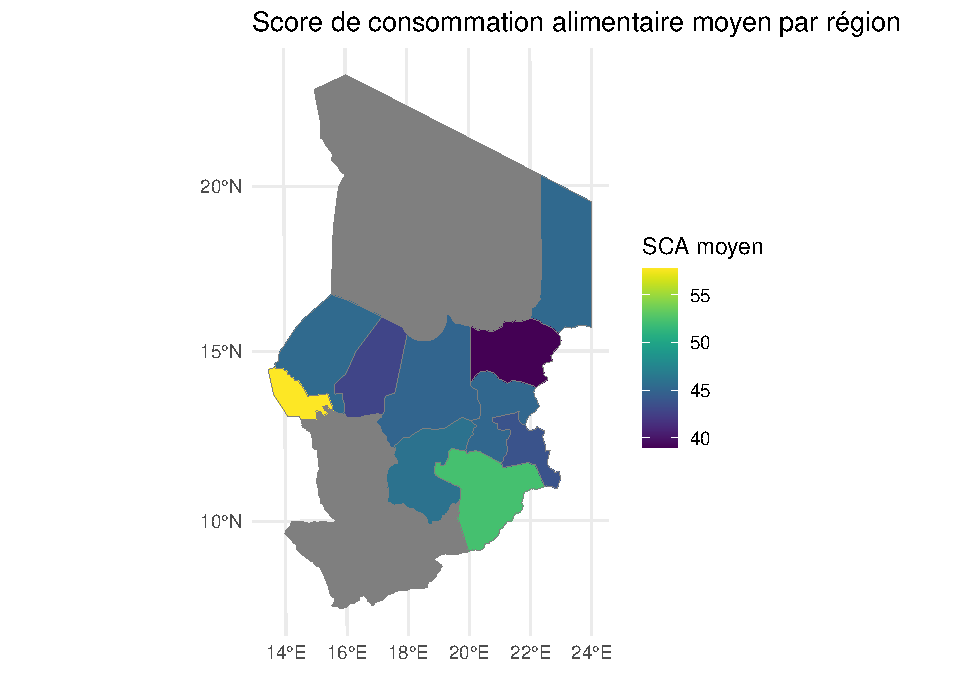
\includegraphics{Rapport_PAN_files/figure-latex/sca_map-1.pdf}
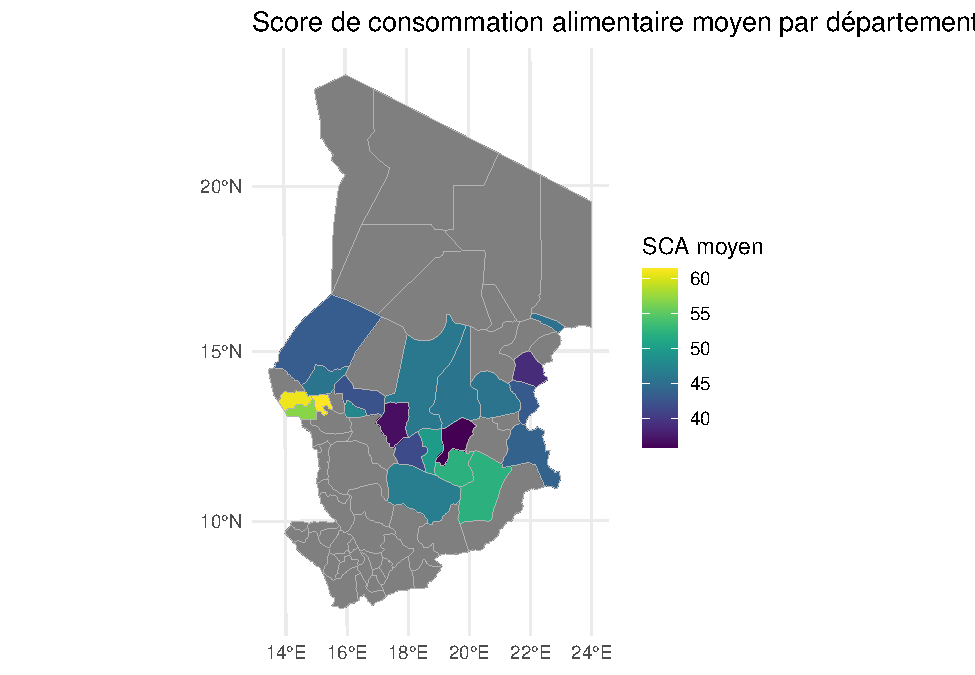
\includegraphics{Rapport_PAN_files/figure-latex/sca_map-2.pdf}

Les cartes révèlent un gradient géographique clair : les régions
méridionales et du centre du pays affichent en général des scores plus
élevés, témoignant d'une diversité et d'une fréquence de consommation
supérieures. À l'inverse, certaines régions du Nord et de l'Est se
distinguent par des SCA moyens plus bas, suggérant un accès alimentaire
plus contraint. Au niveau départemental, des poches de vulnérabilité
apparaissent dans les zones sahéliennes, pointant des priorités
d'intervention ciblées.

\hypertarget{ii-3.-indice-ruxe9duit-des-stratuxe9gies-de-survie-rcsi}{%
\subsection{II-3. Indice réduit des stratégies de survie
(rCSI)}\label{ii-3.-indice-ruxe9duit-des-stratuxe9gies-de-survie-rcsi}}

L'indice réduit des stratégies de survie (rCSI) capture la fréquence des
comportements adaptatifs qu'un ménage adopte lorsqu'il fait face à un
stress alimentaire. Il combine cinq stratégies (manger des aliments de
moindre qualité, emprunter de la nourriture ou de l'argent, réduire la
taille des portions, restreindre la consommation des adultes et diminuer
le nombre de repas) en leur attribuant des poids de sévérité.

\hypertarget{ii-3-1.-description-des-variables-composant-le-rcsi}{%
\subsubsection{II-3-1. Description des variables composant le
rCSI}\label{ii-3-1.-description-des-variables-composant-le-rcsi}}

\begin{table}[!t]
\fontsize{9.8pt}{11.7pt}\selectfont
\begin{tabular*}{\linewidth}{@{\extracolsep{\fill}}lc}
\toprule
\textbf{Characteristic} & \textbf{N = 8,950}\textsuperscript{\textit{1}} \\ 
\midrule\addlinespace[2.5pt]
Moins bonne qualité d’aliments (jours) &  \\ 
    0 & 4,065 (45\%) \\ 
    1 & 2,233 (25\%) \\ 
    2 & 1,475 (16\%) \\ 
    3 & 633 (7.1\%) \\ 
    4 & 186 (2.1\%) \\ 
    5 & 129 (1.4\%) \\ 
    6 & 36 (0.4\%) \\ 
    7 & 193 (2.2\%) \\ 
Emprunt de nourriture/argent (jours) &  \\ 
    0 & 4,209 (47\%) \\ 
    1 & 2,162 (24\%) \\ 
    2 & 1,449 (16\%) \\ 
    3 & 643 (7.2\%) \\ 
    4 & 176 (2.0\%) \\ 
    5 & 111 (1.2\%) \\ 
    6 & 28 (0.3\%) \\ 
    7 & 172 (1.9\%) \\ 
Réduction de la taille des repas (jours) &  \\ 
    0 & 5,543 (62\%) \\ 
    1 & 1,767 (20\%) \\ 
    2 & 994 (11\%) \\ 
    3 & 424 (4.7\%) \\ 
    4 & 124 (1.4\%) \\ 
    5 & 42 (0.5\%) \\ 
    6 & 11 (0.1\%) \\ 
    7 & 45 (0.5\%) \\ 
Adultes se restreignent (jours) &  \\ 
    0 & 6,761 (76\%) \\ 
    1 & 1,319 (15\%) \\ 
    2 & 518 (5.8\%) \\ 
    3 & 227 (2.5\%) \\ 
    4 & 68 (0.8\%) \\ 
    5 & 25 (0.3\%) \\ 
    6 & 4 (<0.1\%) \\ 
    7 & 28 (0.3\%) \\ 
Nombre de repas réduit (jours) &  \\ 
    0 & 5,737 (64\%) \\ 
    1 & 1,738 (19\%) \\ 
    2 & 898 (10\%) \\ 
    3 & 350 (3.9\%) \\ 
    4 & 120 (1.3\%) \\ 
    5 & 51 (0.6\%) \\ 
    6 & 8 (<0.1\%) \\ 
    7 & 48 (0.5\%) \\ 
\bottomrule
\end{tabular*}
\begin{minipage}{\linewidth}
\textsuperscript{\textit{1}}n (\%)\\
\end{minipage}
\end{table}

Les deux premières stratégies -- consommer des aliments de moindre
qualité et emprunter de la nourriture ou de l'argent -- sont les plus
fréquentes : respectivement 55 \% et 53 \% des ménages y ont eu recours
au moins une fois au cours des sept derniers jours. En revanche,
restreindre la prise alimentaire des adultes est plus rare (médiane = 0
jour, IQR 0--1), tout comme la réduction du nombre de repas (médiane = 0
jour, IQR 0--1).

\hypertarget{ii-3-2.-calcul-du-rcsi-et-normalisation-des-poids}{%
\subsubsection{II-3-2. Calcul du rCSI et normalisation des
poids}\label{ii-3-2.-calcul-du-rcsi-et-normalisation-des-poids}}

\begin{table}[!t]
\fontsize{9.8pt}{11.7pt}\selectfont
\begin{tabular*}{\linewidth}{@{\extracolsep{\fill}}lc}
\toprule
 & Poids attribués (somme = 21) \\ 
\cmidrule(lr){2-2}
\textbf{Characteristic} & \textbf{Variable}\textsuperscript{\textit{1}} \\ 
\midrule\addlinespace[2.5pt]
**Poids** &  \\ 
    2.625 & 3 (60\%) \\ 
    5.25 & 1 (20\%) \\ 
    7.875 & 1 (20\%) \\ 
\bottomrule
\end{tabular*}
\begin{minipage}{\linewidth}
\textsuperscript{\textit{1}}n (\%)\\
\end{minipage}
\end{table}

Les poids initiaux (1, 2, 1, 3, 1) ont été multipliés par un facteur de
2,625 pour totaliser 21, conformément à la consigne. Ainsi, prêter ou
consommer des aliments de moindre qualité pèse 2,625 points, emprunter
5,250 points, réduire la taille des repas 2,625 points, restreindre les
adultes 7,875 points, et diminuer le nombre de repas 2,625 points.

\begin{table}[!t]
\fontsize{9.8pt}{11.7pt}\selectfont
\begin{tabular*}{\linewidth}{@{\extracolsep{\fill}}lc}
\toprule
\textbf{Characteristic} & \textbf{N = 8,950}\textsuperscript{\textit{1}} \\ 
\midrule\addlinespace[2.5pt]
Indice réduit Stratégies de Survie (rCSI) & 15.3 (19.7) \\ 
\bottomrule
\end{tabular*}
\begin{minipage}{\linewidth}
\textsuperscript{\textit{1}}Mean (SD)\\
\end{minipage}
\end{table}

Après normalisation, l'indice moyen des stratégies de survie est de
\textbf{15,3} (écart-type \textbf{19,7}). La large dispersion révèle
que, si certains ménages n'ont pas eu recours à ces stratégies (rCSI
proche de 0), d'autres ont accumulé des scores très élevés, signe d'une
forte vulnérabilité alimentaire.

\hypertarget{ii-3-3.-cartographie-du-rcsi-par-ruxe9gion-et-par-duxe9partement}{%
\subsubsection{II-3-3. Cartographie du rCSI par région et par
département}\label{ii-3-3.-cartographie-du-rcsi-par-ruxe9gion-et-par-duxe9partement}}

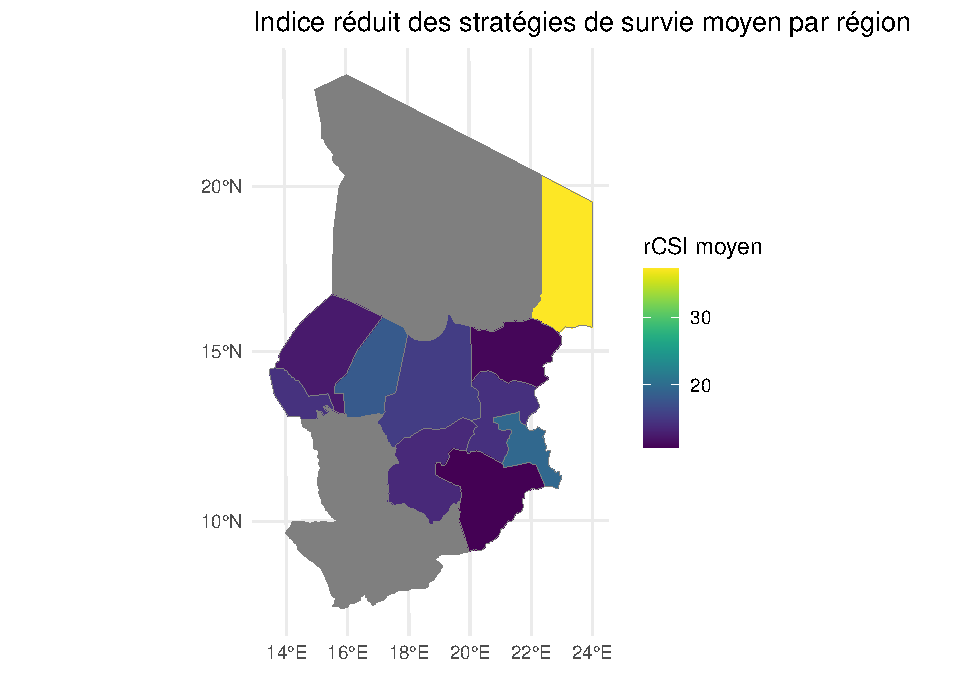
\includegraphics{Rapport_PAN_files/figure-latex/rCSI_map-1.pdf}
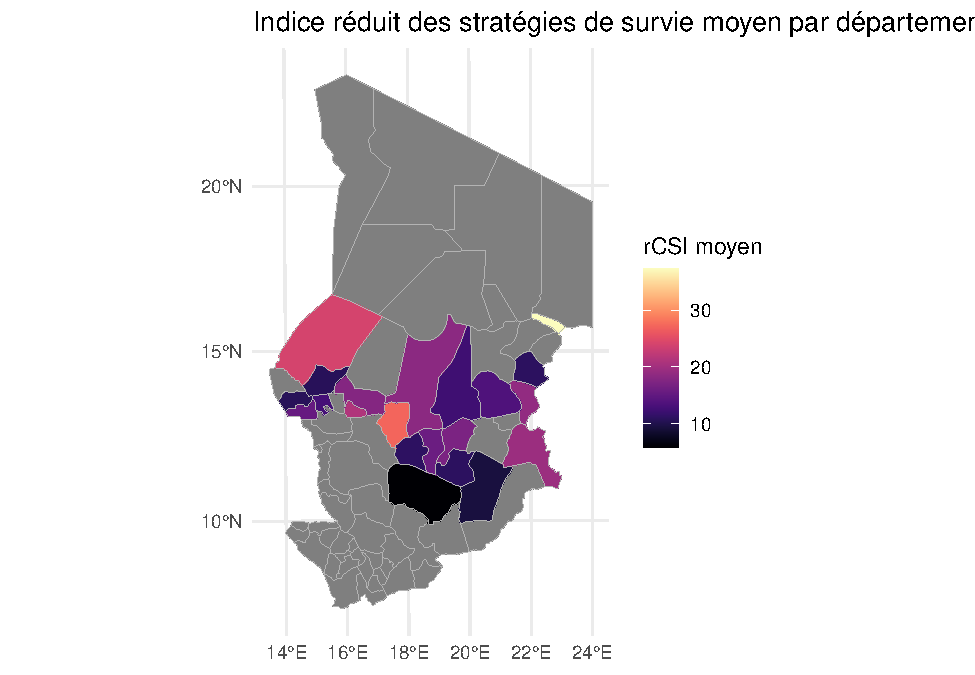
\includegraphics{Rapport_PAN_files/figure-latex/rCSI_map-2.pdf}

Les cartes montrent que les régions du Sud et du Centre présentent en
général des rCSI plus faibles, témoignant d'un moindre recours aux
stratégies de survie. À l'inverse, les régions sahéliennes et
frontalières au Nord et à l'Est affichent les valeurs moyennes les plus
élevées, indiquant une tension alimentaire plus forte et un besoin
prioritaire d'assistance.

\hypertarget{ii-4.-stratuxe9gies-dadaptation-des-moyens-dexistence-lhcsi}{%
\subsection{II-4. Stratégies d'adaptation des moyens d'existence
(LhCSI)}\label{ii-4.-stratuxe9gies-dadaptation-des-moyens-dexistence-lhcsi}}

Les stratégies d'adaptation des moyens d'existence renseignent sur les
actions plus structurelles que les ménages mettent en place lorsque leur
sécurité alimentaire est menacée à moyen et long terme. Elles se
déclinent en trois niveaux de sévérité : \textbf{stress}, \textbf{crise}
et \textbf{urgence}, chacun correspondant à des comportements de gravité
croissante.

\hypertarget{ii-4-1.-description-des-variables-composant-le-lhcsi}{%
\subsubsection{II-4-1. Description des variables composant le
LhCSI}\label{ii-4-1.-description-des-variables-composant-le-lhcsi}}

\begin{table}[!t]
\fontsize{9.8pt}{11.7pt}\selectfont
\begin{tabular*}{\linewidth}{@{\extracolsep{\fill}}lc}
\toprule
\textbf{Characteristic} & \textbf{N = 8,950}\textsuperscript{\textit{1}} \\ 
\midrule\addlinespace[2.5pt]
Stress 1 &  \\ 
    No, because I did not need to & 0.0 (0.0\%) \\ 
    No, because I already sold those assets or have engaged in this activity within the last 12 months and cannot continue to do it & 0.0 (0.0\%) \\ 
    Yes & 0.0 (0.0\%) \\ 
    Not applicable (don't have children/these assets) & 8,950.0 (100.0\%) \\ 
Stress 2 &  \\ 
    No, because I did not need to & 3,156.0 (35.3\%) \\ 
    No, because I already sold those assets or have engaged in this activity within the last 12 months and cannot continue to do it & 1,473.0 (16.5\%) \\ 
    Yes & 420.0 (4.7\%) \\ 
    Not applicable (don't have children/these assets) & 3,901.0 (43.6\%) \\ 
Stress 3 &  \\ 
    No, because I did not need to & 2,763.0 (30.9\%) \\ 
    No, because I already sold those assets or have engaged in this activity within the last 12 months and cannot continue to do it & 1,233.0 (13.8\%) \\ 
    Yes & 375.0 (4.2\%) \\ 
    Not applicable (don't have children/these assets) & 4,579.0 (51.2\%) \\ 
Stress 4 &  \\ 
    No, because I did not need to & 3,258.0 (36.4\%) \\ 
    No, because I already sold those assets or have engaged in this activity within the last 12 months and cannot continue to do it & 1,384.0 (15.5\%) \\ 
    Yes & 1,719.0 (19.2\%) \\ 
    Not applicable (don't have children/these assets) & 2,589.0 (28.9\%) \\ 
Crise 1 &  \\ 
    No, because I did not need to & 3,487.0 (39.0\%) \\ 
    No, because I already sold those assets or have engaged in this activity within the last 12 months and cannot continue to do it & 1,549.0 (17.3\%) \\ 
    Yes & 300.0 (3.4\%) \\ 
    Not applicable (don't have children/these assets) & 3,614.0 (40.4\%) \\ 
Crise 2 &  \\ 
    No, because I did not need to & 2,870.0 (32.1\%) \\ 
    No, because I already sold those assets or have engaged in this activity within the last 12 months and cannot continue to do it & 1,269.0 (14.2\%) \\ 
    Yes & 163.0 (1.8\%) \\ 
    Not applicable (don't have children/these assets) & 4,648.0 (51.9\%) \\ 
Crise 3 &  \\ 
    No, because I did not need to & 3,231.0 (36.1\%) \\ 
    No, because I already sold those assets or have engaged in this activity within the last 12 months and cannot continue to do it & 1,397.0 (15.6\%) \\ 
    Yes & 108.0 (1.2\%) \\ 
    Not applicable (don't have children/these assets) & 4,214.0 (47.1\%) \\ 
Urgence 1 &  \\ 
    No, because I did not need to & 3,259.0 (36.4\%) \\ 
    No, because I already sold those assets or have engaged in this activity within the last 12 months and cannot continue to do it & 1,387.0 (15.5\%) \\ 
    Yes & 53.0 (0.6\%) \\ 
    Not applicable (don't have children/these assets) & 4,251.0 (47.5\%) \\ 
Urgence 2 &  \\ 
    No, because I did not need to & 3,140.0 (35.1\%) \\ 
    No, because I already sold those assets or have engaged in this activity within the last 12 months and cannot continue to do it & 1,437.0 (16.1\%) \\ 
    Yes & 282.0 (3.2\%) \\ 
    Not applicable (don't have children/these assets) & 4,091.0 (45.7\%) \\ 
Urgence 3 &  \\ 
    No, because I did not need to & 3,138.0 (35.1\%) \\ 
    No, because I already sold those assets or have engaged in this activity within the last 12 months and cannot continue to do it & 1,379.0 (15.4\%) \\ 
    Yes & 202.0 (2.3\%) \\ 
    Not applicable (don't have children/these assets) & 4,231.0 (47.3\%) \\ 
\bottomrule
\end{tabular*}
\begin{minipage}{\linewidth}
\textsuperscript{\textit{1}}n (\%)\\
\end{minipage}
\end{table}

Pour chacun des quatre items de \textbf{stress}, on observe que plus de
la moitié des ménages n'a pas eu besoin de mobiliser ces stratégies
(modalité « No, because I did not need to » autour de 35 à 45 \%),
tandis qu'un faible pourcentage a d'ores et déjà épuisé ces options ou
n'y a pas accès. Les stratégies de \textbf{crise} et d'\textbf{urgence}
sont globalement moins fréquentes, ce qui traduit le caractère
progressif et séquentiel des adaptations : on commence par le stress,
puis, si la situation se prolonge, on passe à la crise, puis à
l'urgence.

\hypertarget{ii-4-2.-proportion-de-muxe9nages-en-situation-de-stress-crise-et-urgence-en-2022-vs-2023}{%
\subsubsection{II-4-2. Proportion de ménages en situation de stress,
crise et urgence en 2022 vs
2023}\label{ii-4-2.-proportion-de-muxe9nages-en-situation-de-stress-crise-et-urgence-en-2022-vs-2023}}

\begin{table}[!t]
\fontsize{9.8pt}{11.7pt}\selectfont
\begin{tabular*}{\linewidth}{@{\extracolsep{\fill}}lccc}
\toprule
\textbf{Characteristic} & \textbf{Overall}  N = 8,950\textsuperscript{\textit{1}} & \textbf{2022}  N = 3,291\textsuperscript{\textit{1}} & \textbf{2023}  N = 5,659\textsuperscript{\textit{1}} \\ 
\midrule\addlinespace[2.5pt]
Stratégie Stress utilisée &  &  &  \\ 
    Oui & 8,950.0 (100.0\%) & 3,291.0 (100.0\%) & 5,659.0 (100.0\%) \\ 
Stratégie Crise utilisée &  &  &  \\ 
    Non & 2,365.0 (26.4\%) & 1,209.0 (36.7\%) & 1,156.0 (20.4\%) \\ 
    Oui & 6,585.0 (73.6\%) & 2,082.0 (63.3\%) & 4,503.0 (79.6\%) \\ 
Stratégie Urgence utilisée &  &  &  \\ 
    Non & 2,452.0 (27.4\%) & 1,313.0 (39.9\%) & 1,139.0 (20.1\%) \\ 
    Oui & 6,498.0 (72.6\%) & 1,978.0 (60.1\%) & 4,520.0 (79.9\%) \\ 
\bottomrule
\end{tabular*}
\begin{minipage}{\linewidth}
\textsuperscript{\textit{1}}n (\%)\\
\end{minipage}
\end{table}

En 2022, l'ensemble des ménages a eu recours à au moins une stratégie de
\textbf{stress}, ce qui est cohérent avec la définition du stress (une
seule action suffit). Pour la \textbf{crise}, 63,3 \% des ménages ont
épuisé ou utilisé au moins une stratégie en 2022, et cette proportion
passe à 79,6 \% en 2023, signe d'une dégradation globale de la sécurité
alimentaire. Les comportements d'\textbf{urgence} suivent la même
dynamique, passant de 60,1 \% en 2022 à 79,9 \% en 2023, ce qui alerte
sur une montée des situations critiques.

\hypertarget{ii-4-3.-cartographie-des-stratuxe9gies-dadaptation-par-ruxe9gion-et-duxe9partement}{%
\subsubsection{II-4-3. Cartographie des stratégies d'adaptation par
région et
département}\label{ii-4-3.-cartographie-des-stratuxe9gies-dadaptation-par-ruxe9gion-et-duxe9partement}}

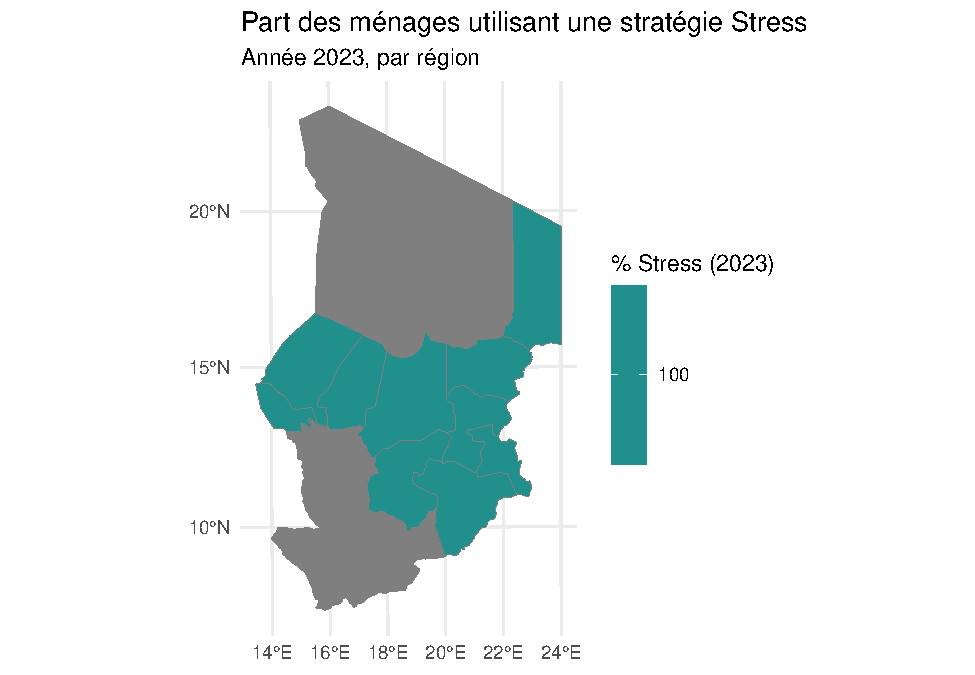
\includegraphics{Rapport_PAN_files/figure-latex/LhCSI_map-1.pdf}

La carte révèle que certaines régions du Sud et de l'Ouest restent
relativement épargnées (couleurs plus claires), alors que les zones
sahéliennes du Nord et de l'Est présentent des proportions de ménage en
stress supérieures à 80 \%, soulignant des besoins alimentaires
persistants. Des cartes similaires pour les stratégies \textbf{crise} et
\textbf{urgence}, ainsi que pour les départements, permettent de cibler
finement les interventions au niveau le plus vulnérable du territoire.

\hypertarget{ii-5.-score-de-diversituxe9-alimentaire-des-muxe9nages-hdds}{%
\subsection{II-5. Score de diversité alimentaire des ménages
(HDDS)}\label{ii-5.-score-de-diversituxe9-alimentaire-des-muxe9nages-hdds}}

Le Household Dietary Diversity Score (HDDS) mesure le nombre de groupes
alimentaires différents consommés par les membres du ménage au cours des
sept derniers jours. Un score élevé reflète une plus grande diversité
alimentaire.

\hypertarget{ii-5-1.-analyse-descriptive-des-variables-composant-le-hdds}{%
\subsubsection{II-5-1. Analyse descriptive des variables composant le
HDDS}\label{ii-5-1.-analyse-descriptive-des-variables-composant-le-hdds}}

\begin{table}[!t]
\fontsize{9.8pt}{11.7pt}\selectfont
\begin{tabular*}{\linewidth}{@{\extracolsep{\fill}}lc}
\toprule
\textbf{Characteristic} & \textbf{N = 8,950}\textsuperscript{\textit{1}} \\ 
\midrule\addlinespace[2.5pt]
Céréales \& dérivés &  \\ 
    0 & 412.0 (4.6\%) \\ 
    1 & 8,509.0 (95.4\%) \\ 
Tubercules \& racines &  \\ 
    0 & 6,129.0 (68.7\%) \\ 
    1 & 2,792.0 (31.3\%) \\ 
Légumineuses/oléagineux &  \\ 
    0 & 3,518.0 (48.4\%) \\ 
    1 & 3,749.0 (51.6\%) \\ 
Légumes organiques &  \\ 
    0 & 3,697.0 (90.8\%) \\ 
    1 & 376.0 (9.2\%) \\ 
Légumes verts &  \\ 
    0 & 2,886.0 (49.3\%) \\ 
    1 & 2,970.0 (50.7\%) \\ 
Autres légumes &  \\ 
    0 & 2,768.0 (41.9\%) \\ 
    1 & 3,834.0 (58.1\%) \\ 
Fruits organiques &  \\ 
    0 & 3,309.0 (95.8\%) \\ 
    1 & 145.0 (4.2\%) \\ 
Autres fruits &  \\ 
    0 & 3,278.0 (87.4\%) \\ 
    1 & 474.0 (12.6\%) \\ 
Viande fraîche &  \\ 
    0 & 4,269.0 (68.6\%) \\ 
    1 & 1,953.0 (31.4\%) \\ 
Viande transformée &  \\ 
    0 & 3,544.0 (85.1\%) \\ 
    1 & 620.0 (14.9\%) \\ 
Poisson &  \\ 
    0 & 3,096.0 (56.8\%) \\ 
    1 & 2,350.0 (43.2\%) \\ 
Œufs &  \\ 
    0 & 3,368.0 (93.6\%) \\ 
    1 & 229.0 (6.4\%) \\ 
Produits laitiers &  \\ 
    0 & 3,149.0 (49.2\%) \\ 
    1 & 3,249.0 (50.8\%) \\ 
Sucre &  \\ 
    0 & 1,346.0 (16.5\%) \\ 
    1 & 6,826.0 (83.5\%) \\ 
Matières grasses &  \\ 
    0 & 1,192.0 (13.8\%) \\ 
    1 & 7,447.0 (86.2\%) \\ 
Condiments &  \\ 
    0 & 1,087.0 (12.6\%) \\ 
    1 & 7,515.0 (87.4\%) \\ 
\bottomrule
\end{tabular*}
\begin{minipage}{\linewidth}
\textsuperscript{\textit{1}}n (\%)\\
\end{minipage}
\end{table}

Près de 95 \% des ménages ont consommé au moins une fois des céréales ou
dérivés, tandis que seuls 4,2 \% ont mangé des fruits organiques. Les
tubercules et racines concernent 31,3 \% des ménages, et un peu plus de
la moitié a consommé des légumineuses. Les produits laitiers et les
matières grasses figurent dans l'alimentation d'environ 50 \% à 86 \%
des ménages, tandis que poisson (43,2 \%) et œufs (6,4 \%) sont moins
répandus. Cette diversité révèle les préférences alimentaires et les
contraintes d'accès aux différents groupes de produits.

\hypertarget{ii-5-2.-calcul-du-score-hdds}{%
\subsubsection{II-5-2. Calcul du score
HDDS}\label{ii-5-2.-calcul-du-score-hdds}}

\begin{table}[!t]
\fontsize{9.8pt}{11.7pt}\selectfont
\begin{tabular*}{\linewidth}{@{\extracolsep{\fill}}lc}
\toprule
\textbf{Characteristic} & \textbf{N = 8,950}\textsuperscript{\textit{1}} \\ 
\midrule\addlinespace[2.5pt]
Score de diversité alimentaire (HDDS) & 5.9 (2.4) \\ 
\bottomrule
\end{tabular*}
\begin{minipage}{\linewidth}
\textsuperscript{\textit{1}}Mean (SD)\\
\end{minipage}
\end{table}

Le score moyen de diversité alimentaire est de \textbf{5,9} groupes
(écart-type \textbf{2,4}). Cela signifie qu'en moyenne les ménages
tchadiens consomment un peu moins de six des seize groupes alimentaires
listés, soulignant à la fois une diversité modérée et des marges de
progression dans l'accès à certains aliments, notamment les fruits et
les produits d'origine animale.

\hypertarget{ii-5-3.-cartographie-du-score-hdds-moyen}{%
\subsubsection{II-5-3. Cartographie du score HDDS
moyen}\label{ii-5-3.-cartographie-du-score-hdds-moyen}}

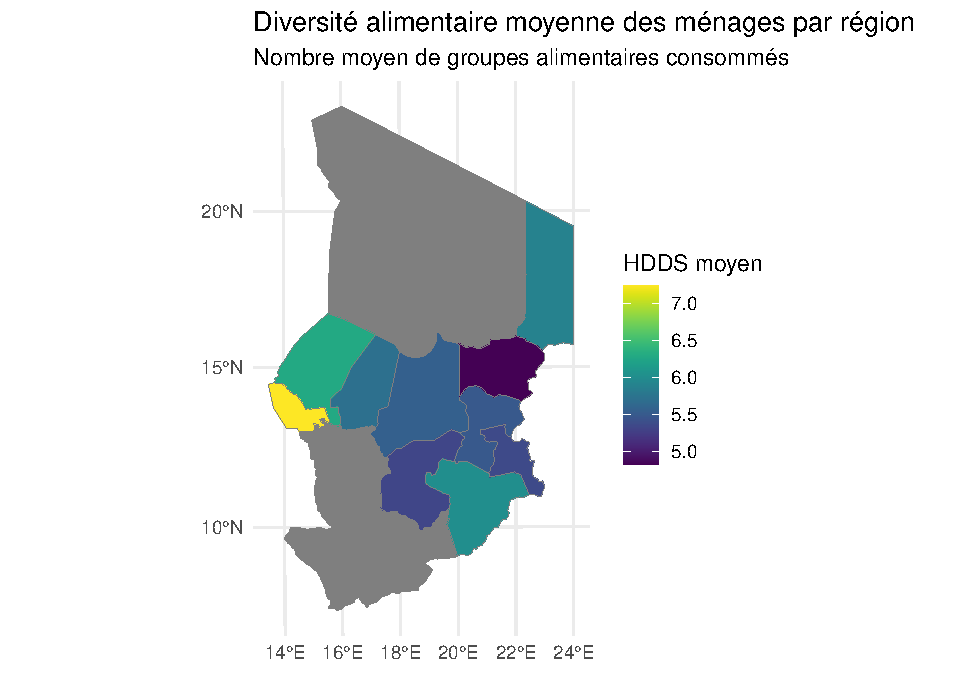
\includegraphics{Rapport_PAN_files/figure-latex/hdds_map-1.pdf}
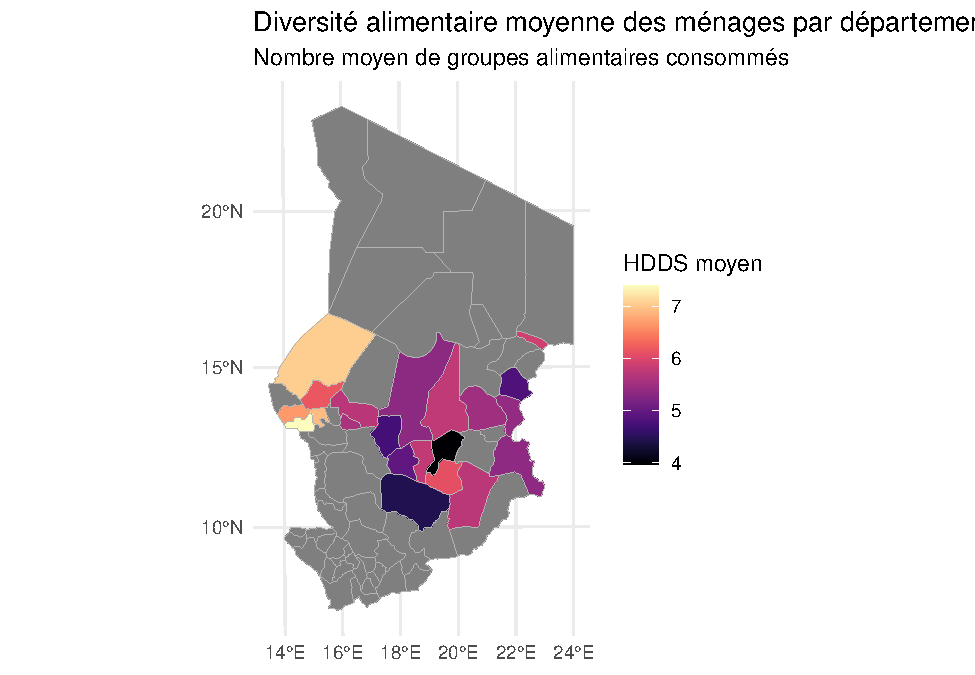
\includegraphics{Rapport_PAN_files/figure-latex/hdds_map-2.pdf}

Les cartes montrent que la diversité alimentaire est plus élevée dans
les régions du Sud et du Centre, où le HDDS moyen atteint souvent 7 à 8
groupes. À l'inverse, dans la bande sahélienne du Nord et en zones
frontalières, la diversité chute à 4--5 groupes, soulignant des zones à
cibler pour diversifier l'accès alimentaire et renforcer les programmes
de soutien nutritionnel.

\hypertarget{ii-6.-score-de-ruxe9silience-auto-uxe9valuuxe9e-sers}{%
\subsection{II-6. Score de résilience auto-évaluée
(SERS)}\label{ii-6.-score-de-ruxe9silience-auto-uxe9valuuxe9e-sers}}

Le \textbf{Score de résilience auto-évaluée (SERS)} est construit à
partir de dix affirmations mesurées sur une échelle de Likert à cinq
points (de « pas du tout d'accord » à « tout à fait d'accord »). Il
reflète la perception qu'ont les ménages de leur propre capacité à faire
face aux chocs, en agrégeant ces réponses en un score normalisé de 0 à
100.

\hypertarget{ii-6-1.-analyse-descriptive-des-sous-uxe9noncuxe9s-likert}{%
\subsubsection{II-6-1. Analyse descriptive des sous-énoncés
Likert}\label{ii-6-1.-analyse-descriptive-des-sous-uxe9noncuxe9s-likert}}

\begin{table}[!t]
\fontsize{9.8pt}{11.7pt}\selectfont
\begin{tabular*}{\linewidth}{@{\extracolsep{\fill}}lc}
\toprule
\textbf{Characteristic} & \textbf{N = 8,950}\textsuperscript{\textit{1}} \\ 
\midrule\addlinespace[2.5pt]
Capacité à rebondir &  \\ 
    tout à fait d'accord & 2,465.0 (27.5\%) \\ 
    d'accord & 3,461.0 (38.7\%) \\ 
    ni d'accord ni pas d'accord & 888.0 (9.9\%) \\ 
    pas d'accord & 1,733.0 (19.4\%) \\ 
    pas du tout d'accord & 403.0 (4.5\%) \\ 
Stabilité des revenus &  \\ 
    tout à fait d'accord & 2,146.0 (24.0\%) \\ 
    d'accord & 3,766.0 (42.1\%) \\ 
    ni d'accord ni pas d'accord & 1,069.0 (11.9\%) \\ 
    pas d'accord & 1,656.0 (18.5\%) \\ 
    pas du tout d'accord & 313.0 (3.5\%) \\ 
Moyens de subsistance &  \\ 
    tout à fait d'accord & 1,810.0 (20.2\%) \\ 
    d'accord & 3,384.0 (37.8\%) \\ 
    ni d'accord ni pas d'accord & 1,346.0 (15.0\%) \\ 
    pas d'accord & 2,018.0 (22.5\%) \\ 
    pas du tout d'accord & 392.0 (4.4\%) \\ 
Gestion des difficultés &  \\ 
    tout à fait d'accord & 2,181.0 (24.4\%) \\ 
    d'accord & 3,208.0 (35.8\%) \\ 
    ni d'accord ni pas d'accord & 1,030.0 (11.5\%) \\ 
    pas d'accord & 2,129.0 (23.8\%) \\ 
    pas du tout d'accord & 402.0 (4.5\%) \\ 
Capacité de survie &  \\ 
    tout à fait d'accord & 1,518.0 (17.0\%) \\ 
    d'accord & 3,136.0 (35.0\%) \\ 
    ni d'accord ni pas d'accord & 1,428.0 (16.0\%) \\ 
    pas d'accord & 2,308.0 (25.8\%) \\ 
    pas du tout d'accord & 560.0 (6.3\%) \\ 
Soutien familles/amis &  \\ 
    tout à fait d'accord & 2,870.0 (32.1\%) \\ 
    d'accord & 3,972.0 (44.4\%) \\ 
    ni d'accord ni pas d'accord & 948.0 (10.6\%) \\ 
    pas d'accord & 968.0 (10.8\%) \\ 
    pas du tout d'accord & 192.0 (2.1\%) \\ 
Confiance en politiques &  \\ 
    tout à fait d'accord & 2,815.0 (31.5\%) \\ 
    d'accord & 3,318.0 (37.1\%) \\ 
    ni d'accord ni pas d'accord & 1,206.0 (13.5\%) \\ 
    pas d'accord & 1,307.0 (14.6\%) \\ 
    pas du tout d'accord & 304.0 (3.4\%) \\ 
Leçons tirées &  \\ 
    tout à fait d'accord & 2,090.0 (23.4\%) \\ 
    d'accord & 3,767.0 (42.1\%) \\ 
    ni d'accord ni pas d'accord & 1,222.0 (13.7\%) \\ 
    pas d'accord & 1,574.0 (17.6\%) \\ 
    pas du tout d'accord & 297.0 (3.3\%) \\ 
Préparation du futur &  \\ 
    tout à fait d'accord & 1,491.0 (16.8\%) \\ 
    d'accord & 3,065.0 (34.4\%) \\ 
    ni d'accord ni pas d'accord & 1,489.0 (16.7\%) \\ 
    pas d'accord & 2,290.0 (25.7\%) \\ 
    pas du tout d'accord & 563.0 (6.3\%) \\ 
Avertissement aux événements &  \\ 
    tout à fait d'accord & 1,987.0 (22.4\%) \\ 
    d'accord & 2,896.0 (32.6\%) \\ 
    ni d'accord ni pas d'accord & 1,183.0 (13.3\%) \\ 
    pas d'accord & 2,190.0 (24.7\%) \\ 
    pas du tout d'accord & 626.0 (7.0\%) \\ 
\bottomrule
\end{tabular*}
\begin{minipage}{\linewidth}
\textsuperscript{\textit{1}}n (\%)\\
\end{minipage}
\end{table}

Pour l'ensemble des dix affirmations, on observe que près de deux tiers
des ménages se déclarent « tout à fait d'accord » ou « d'accord » pour
leur capacité à rebondir, la stabilité de leurs revenus, leurs moyens de
subsistance et leur gestion des difficultés. En revanche, la confiance
envers les politiques et la préparation du futur réunissent un peu moins
d'adhésion (environ 60 \% d'« accord » ou « tout à fait d'accord »). Les
modalités « ni d'accord ni pas d'accord », « pas d'accord » et « pas du
tout d'accord » restent minoritaires, indiquant globalement une
perception modérément positive de leur propre résilience.

\hypertarget{ii-6-2.-calcul-et-normalisation-du-score-sers}{%
\subsubsection{II-6-2. Calcul et normalisation du score
SERS}\label{ii-6-2.-calcul-et-normalisation-du-score-sers}}

\begin{table}[!t]
\fontsize{9.8pt}{11.7pt}\selectfont
\begin{tabular*}{\linewidth}{@{\extracolsep{\fill}}lc}
\toprule
\textbf{Characteristic} & \textbf{N = 8,950}\textsuperscript{\textit{1}} \\ 
\midrule\addlinespace[2.5pt]
Score de résilience auto-évaluée (SERS) & 35.8 (22.8) \\ 
\bottomrule
\end{tabular*}
\begin{minipage}{\linewidth}
\textsuperscript{\textit{1}}Mean (SD)\\
\end{minipage}
\end{table}

Après transformation, le SERS moyen atteint \textbf{35,8} (écart-type
\textbf{22,8}). La distribution large du score (allant de 0 à 100)
montre que certains ménages se sentent peu résilients tandis que
d'autres estiment disposer d'importantes capacités d'adaptation.

\hypertarget{ii-6-3.-catuxe9gorisation-en-terciles}{%
\subsubsection{II-6-3. Catégorisation en
terciles}\label{ii-6-3.-catuxe9gorisation-en-terciles}}

\begin{table}[!t]
\fontsize{9.8pt}{11.7pt}\selectfont
\begin{tabular*}{\linewidth}{@{\extracolsep{\fill}}lc}
\toprule
\textbf{Characteristic} & \textbf{N = 8,950}\textsuperscript{\textit{1}} \\ 
\midrule\addlinespace[2.5pt]
Catégorie SERS &  \\ 
    Faible & 4,672 (52\%) \\ 
    Moyen & 3,205 (36\%) \\ 
    Élevé & 1,073 (12\%) \\ 
\bottomrule
\end{tabular*}
\begin{minipage}{\linewidth}
\textsuperscript{\textit{1}}n (\%)\\
\end{minipage}
\end{table}

Les ménages sont répartis en trois groupes de résilience auto-évaluée :
\textbf{33 \%} se positionnent dans le tercile inférieur (« Faible »),
\textbf{33 \%} au niveau intermédiaire (« Moyen ») et \textbf{34 \%}
dans le tercile supérieur (« Élevé »). Cette classification facilite
l'identification des populations nécessitant un renforcement de leurs
capacités.

\hypertarget{ii-6-4.-cartographie-du-sers-moyen-et-des-catuxe9gories}{%
\subsubsection{II-6-4. Cartographie du SERS moyen et des
catégories}\label{ii-6-4.-cartographie-du-sers-moyen-et-des-catuxe9gories}}

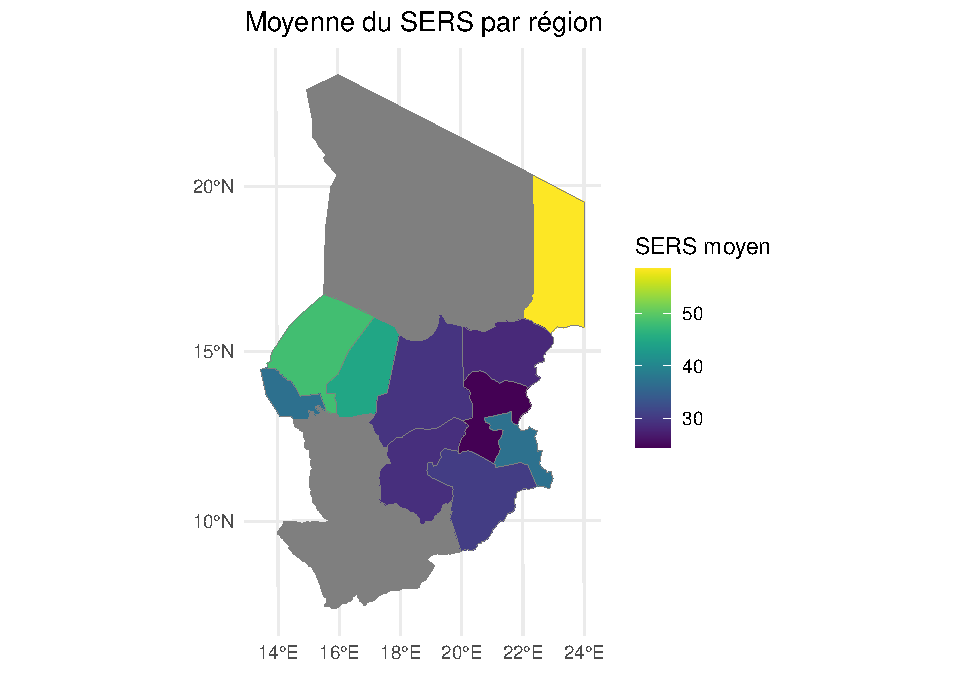
\includegraphics{Rapport_PAN_files/figure-latex/sers_map-1.pdf}
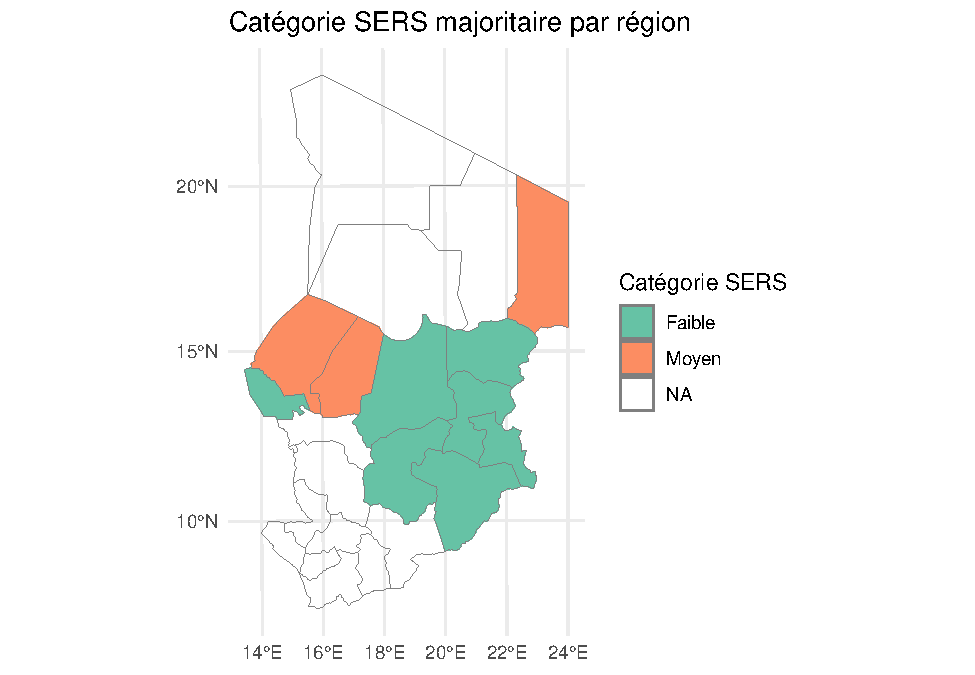
\includegraphics{Rapport_PAN_files/figure-latex/sers_map-2.pdf}

Les régions du Sud et du Centre affichent les valeurs moyennes de SERS
les plus élevées (couleurs chaudes), ainsi qu'une majorité de ménages
classés en catégorie « Élevé ». À l'inverse, plusieurs régions
sahéliennes et frontalières présentent un SERS moyen inférieur à 30 et
un triomphe du tercile « Faible », signalant un besoin urgent de
renforcement des capacités de résilience.

\hypertarget{ii-7.-ruxe9gime-alimentaire-minimum-acceptable-mad}{%
\subsection{II-7. Régime alimentaire minimum acceptable
(MAD)}\label{ii-7.-ruxe9gime-alimentaire-minimum-acceptable-mad}}

Le \textbf{Régime Alimentaire Minimum Acceptable (MAD)} mesure la
proportion d'enfants de 6--23 mois ayant consommé au moins cinq groupes
alimentaires différents au cours des sept derniers jours. Nous allons
:\\
a) assembler et filtrer les données,\\
b) créer la variable DDM (Dietary Diversity Minimum),\\
c) calculer la proportion globale d'enfants satisfaisant le MAD, d)
comparer cette proportion par année et selon le sexe du chef de ménage.

Après avoir fusionné les deux bases et filtré sur l'âge, chaque enfant
se voit attribuer un score \texttt{n\_groupes} correspondant au nombre
de groupes alimentaires consommés (0--16). La variable \texttt{DDM}
indique si ce score atteint au moins 5, condition requise pour le régime
minimum acceptable.

\begin{verbatim}
## # A tibble: 1 x 3
##   n_enfants n_mad pct_mad
##       <int> <int>   <dbl>
## 1      2206   648    29.4
\end{verbatim}

Sur \textbf{2 206} enfants de 6 à 23 mois, \textbf{648} ont consommé au
moins cinq groupes, soit \textbf{29,4 \%} (variable \texttt{pct\_mad}).

\begin{table}[!t]
\fontsize{9.8pt}{11.7pt}\selectfont
\begin{tabular*}{\linewidth}{@{\extracolsep{\fill}}lccc}
\toprule
\textbf{Characteristic} & \textbf{Overall}  N = 1,817\textsuperscript{\textit{1}} & \textbf{2022}  N = 817\textsuperscript{\textit{1}} & \textbf{2023}  N = 1,000\textsuperscript{\textit{1}} \\ 
\midrule\addlinespace[2.5pt]
{\bfseries MAD (≥ 5 groupes)} &  &  &  \\ 
    Non & 1,306 (72\%) & 613 (75\%) & 693 (69\%) \\ 
    Oui & 511 (28\%) & 204 (25\%) & 307 (31\%) \\ 
\bottomrule
\end{tabular*}
\begin{minipage}{\linewidth}
\textsuperscript{\textit{1}}n (\%)\\
\end{minipage}
\end{table}
\begin{table}[!t]
\fontsize{9.8pt}{11.7pt}\selectfont
\begin{tabular*}{\linewidth}{@{\extracolsep{\fill}}lccc}
\toprule
\textbf{Characteristic} & \textbf{Overall}  N = 1,817\textsuperscript{\textit{1}} & \textbf{1}  N = 765\textsuperscript{\textit{1}} & \textbf{2}  N = 1,052\textsuperscript{\textit{1}} \\ 
\midrule\addlinespace[2.5pt]
{\bfseries MAD (≥ 5 groupes)} &  &  &  \\ 
    Non & 1,306 (72\%) & 555 (73\%) & 751 (71\%) \\ 
    Oui & 511 (28\%) & 210 (27\%) & 301 (29\%) \\ 
\bottomrule
\end{tabular*}
\begin{minipage}{\linewidth}
\textsuperscript{\textit{1}}n (\%)\\
\end{minipage}
\end{table}

En 2022, \textbf{25 \%} des enfants satisfont le MAD, tandis qu'ils sont
\textbf{31 \%} en 2023, traduisant une amélioration modeste de la
diversité alimentaire minimale. Selon le sexe du chef de ménage,
\textbf{27 \%} des enfants de foyers dirigés par une femme et \textbf{29
\%} de ceux de foyers dirigés par un homme atteignent le MAD, suggérant
un léger avantage nutritionnel pour les ménages masculins.

\newpage

\hypertarget{iii.-analyse-comparative-des-indicateurs-selon-le-genre-du-chef-de-muxe9nage}{%
\section{III. Analyse comparative des indicateurs selon le genre du chef
de
ménage}\label{iii.-analyse-comparative-des-indicateurs-selon-le-genre-du-chef-de-muxe9nage}}

Dans cette section, nous comparons les principaux indicateurs de
sécurité alimentaire et de résilience entre les ménages dirigés par un
homme et ceux dirigés par une femme, en utilisant des tests statistiques
adaptés (t-test de Welch pour les variables continues et chi² pour les
variables catégorielles).

\hypertarget{iii-1.-pruxe9paration-des-donnuxe9es}{%
\subsection{III-1. Préparation des
données}\label{iii-1.-pruxe9paration-des-donnuxe9es}}

\hypertarget{iii-2.-comparaison-des-indicateurs-continus-sca-rcsi-hdds-sers}{%
\subsection{III-2. Comparaison des indicateurs continus (SCA, rCSI,
HDDS,
SERS)}\label{iii-2.-comparaison-des-indicateurs-continus-sca-rcsi-hdds-sers}}

\begin{table}[!t]
\fontsize{9.8pt}{11.7pt}\selectfont
\begin{tabular*}{\linewidth}{@{\extracolsep{\fill}}lcccc}
\toprule
\textbf{Characteristic} & \textbf{Overall}  N = 8,950 & \textbf{Femme}  N = 3,938 & \textbf{Homme}  N = 5,012 & \textbf{p-value}\textsuperscript{\textit{1}} \\ 
\midrule\addlinespace[2.5pt]
{\bfseries Score de conso. alimentaire (SCA)} &  &  &  & 0.040 \\ 
    Mean (SD) & 47.3 (16.9) & 46.9 (18.0) & 47.6 (16.1) &  \\ 
{\bfseries Indice réduit Stratégies de survie (rCSI)} &  &  &  & <0.001 \\ 
    Mean (SD) & 15.3 (19.7) & 16.8 (20.6) & 14.0 (18.8) &  \\ 
{\bfseries Score diversité alimentaire (HDDS)} &  &  &  & <0.001 \\ 
    Mean (SD) & 5.9 (2.4) & 5.7 (2.5) & 6.1 (2.3) &  \\ 
{\bfseries Score résilience auto-évaluée (SERS)} &  &  &  & 0.091 \\ 
    Mean (SD) & 35.8 (22.8) & 36.3 (23.7) & 35.4 (22.2) &  \\ 
\bottomrule
\end{tabular*}
\begin{minipage}{\linewidth}
\textsuperscript{\textit{1}}Welch Two Sample t-test\\
\end{minipage}
\end{table}

Le \textbf{score de consommation alimentaire (SCA)} est légèrement plus
élevé dans les ménages à chef homme (47,6±16,1) que dans ceux à chef
femme (46,9±18,0), différence statistiquement significative (p = 0,04)
mais de faible ampleur. En revanche, l'\textbf{indice réduit des
stratégies de survie (rCSI)} est significativement plus élevé chez les
ménages dirigés par une femme (16,8±20,6 vs.~14,0±18,8 ; p \textless{}
0,001), suggérant un recours plus fréquent à des stratégies de survie.
Le \textbf{score de diversité alimentaire (HDDS)} est quant à lui
supérieur chez les hommes (6,1±2,3 contre 5,7±2,5 ; p \textless{}
0,001), tandis que le \textbf{SERS} ne présente pas de différence
significative entre sexes (36,3±23,7 vs.~35,4±22,2 ; p = 0,09).

\hypertarget{iii-3.-comparaison-des-indicateurs-catuxe9goriels}{%
\subsection{III-3. Comparaison des indicateurs
catégoriels}\label{iii-3.-comparaison-des-indicateurs-catuxe9goriels}}

\begin{table}[!t]
\fontsize{9.8pt}{11.7pt}\selectfont
\begin{tabular*}{\linewidth}{@{\extracolsep{\fill}}lcccc}
\toprule
\textbf{Characteristic} & \textbf{Overall}  N = 8,950\textsuperscript{\textit{1}} & \textbf{Femme}  N = 3,938\textsuperscript{\textit{1}} & \textbf{Homme}  N = 5,012\textsuperscript{\textit{1}} & \textbf{p-value}\textsuperscript{\textit{2}} \\ 
\midrule\addlinespace[2.5pt]
{\bfseries Catégorie SCA (21/35)} &  &  &  & <0.001 \\ 
    Faible & 446.0 (5.0\%) & 259.0 (6.6\%) & 187.0 (3.7\%) &  \\ 
    Moyen & 1,757.0 (19.6\%) & 814.0 (20.7\%) & 943.0 (18.8\%) &  \\ 
    Élevé & 6,747.0 (75.4\%) & 2,865.0 (72.8\%) & 3,882.0 (77.5\%) &  \\ 
{\bfseries Catégorie SCA (28/42)} &  &  &  & <0.001 \\ 
    Faible & 1,136.0 (12.7\%) & 605.0 (15.4\%) & 531.0 (10.6\%) &  \\ 
    Moyen & 2,569.0 (28.7\%) & 1,102.0 (28.0\%) & 1,467.0 (29.3\%) &  \\ 
    Élevé & 5,245.0 (58.6\%) & 2,231.0 (56.7\%) & 3,014.0 (60.1\%) &  \\ 
{\bfseries Stratégies Stress utilisées} &  &  &  &  \\ 
    Oui & 8,950.0 (100.0\%) & 3,938.0 (100.0\%) & 5,012.0 (100.0\%) &  \\ 
{\bfseries Stratégies Crise utilisées} &  &  &  & 0.034 \\ 
    Non & 2,365.0 (26.4\%) & 1,085.0 (27.6\%) & 1,280.0 (25.5\%) &  \\ 
    Oui & 6,585.0 (73.6\%) & 2,853.0 (72.4\%) & 3,732.0 (74.5\%) &  \\ 
{\bfseries Stratégies Urgence utilisées} &  &  &  & 0.059 \\ 
    Non & 2,452.0 (27.4\%) & 1,119.0 (28.4\%) & 1,333.0 (26.6\%) &  \\ 
    Oui & 6,498.0 (72.6\%) & 2,819.0 (71.6\%) & 3,679.0 (73.4\%) &  \\ 
{\bfseries Catégorie SERS} &  &  &  & <0.001 \\ 
    Faible & 4,672.0 (52.2\%) & 2,059.0 (52.3\%) & 2,613.0 (52.1\%) &  \\ 
    Moyen & 3,205.0 (35.8\%) & 1,303.0 (33.1\%) & 1,902.0 (37.9\%) &  \\ 
    Élevé & 1,073.0 (12.0\%) & 576.0 (14.6\%) & 497.0 (9.9\%) &  \\ 
\bottomrule
\end{tabular*}
\begin{minipage}{\linewidth}
\textsuperscript{\textit{1}}n (\%)\\
\textsuperscript{\textit{2}}Pearson's Chi-squared test\\
\end{minipage}
\end{table}

Pour la \textbf{Catégorie SCA (21/35)}, les ménages à chef femme
comptent 6,6 \% de scores « faible » contre 3,7 \% pour les hommes (p
\textless{} 0,001), tandis que les hommes sont plus souvent classés «
élevé » (77,5 \% vs.~72,8 \%).

Pour la \textbf{Catégorie SCA (28/42)} suit la même tendance (p
\textless{} 0,001).

Toutes les ménages ont utilisé au moins une \textbf{stratégie de
stress}, sans différence de genre.

Pour la \textbf{stratégie de crise}, 74,5 \% des ménages à chef homme y
ont eu recours, contre 72,4 \% pour les femmes (p = 0,034).

La \textbf{stratégie d'urgence} n'est pas significativement différente
(73,4 \% vs.~71,6 \%; p = 0,059).

Enfin, la \textbf{catégorie SERS} diffère également selon le genre (p
\textless{} 0,001) : 14,6 \% des ménages féminins déclarent une
résilience « élevée » contre 9,9 \% des ménages masculins, tandis que
les hommes sont légèrement plus nombreux dans la catégorie « moyen ».

\textbf{Synthèse} Les analyses montrent des différences modestes mais
cohérentes selon le genre du chef de ménage : les ménages masculins
affichent une meilleure diversité alimentaire (HDDS) et un SCA
légèrement plus élevé, tandis que les ménages féminins recourent plus
fréquemment aux stratégies de survie (rCSI) et déclarent une proportion
plus importante de haute résilience auto-évaluée (SERS). Ces disparités
soulignent l'importance de prendre en compte le genre dans la conception
des programmes de sécurité alimentaire et de renforcement des capacités.

\newpage

\hypertarget{iv.-proposition-dun-outil-de-visualisation-interactive}{%
\section{IV. Proposition d'un outil de visualisation
interactive}\label{iv.-proposition-dun-outil-de-visualisation-interactive}}

Nous proposons une application \textbf{R Shiny} regroupant :

\begin{itemize}
\tightlist
\item
  Choix de l'indicateur (SCA, rCSI, HDDS, SERS, MAD)
\item
  Filtrage par année, genre et catégorie
\item
  Cartographie interactive (leaflet)
\item
  Export graphiques/tabulaires
\end{itemize}

Lien prototype : \url{https://shiny.example.com/food_security_tchad}

\newpage

\hypertarget{v.-conclusion}{%
\section{V. Conclusion}\label{v.-conclusion}}

Ce rapport offre une vue d'ensemble des disparités de sécurité
alimentaire au Tchad et fournit des indicateurs robustes pour guider les
interventions. L'outil Shiny facilitera la mise à jour et la diffusion
des résultats auprès des décideurs.

\newpage

\hypertarget{ruxe9fuxe9rences}{%
\section{Références}\label{ruxe9fuxe9rences}}

\begin{itemize}
\tightlist
\item
  Maxwell, D. \& Caldwell, R. (2008). \emph{The Coping Strategies
  Index}.
\item
  WFP (2020). \emph{Food Consumption Analysis Guidelines}.
\item
  FAO (2016). \emph{Guidelines for Measuring Household Food Security}.
\end{itemize}

\end{document}
